\section{Funcionamiento de los m\'etodos de estabilidad de laderas en Scoops3D}



Como se ha mencionado anteriormente, Scoops3D se basa en la aplicaci\'on de los an\'alisis de equilibrio l\'imite por medio de los m\'etodos de de dobelas, que aplicado en un entorno tridimensional puede verse como una an\'alisis por medio de columnas.
Cada columna posee entonces lados de distancia equivalente, dados por el tama\~no de pixel que posee el DEM especificado, mientras que la altura de la columna estar\'a dada por la distancia entre la superficie del DEM y la superficie de falla.

La superficie de falla que intersecta las dobelas en profundidad es una esfera con centro en cualquier lugar sobre la superficie del DEM y un radio \textit{r}. Scoops3D incluye en el an\'alisis de cada superficie de falla todas y cada una de las columnas cuyo p\'ixel correspondiente posea 2 o mas v\'ertices al interior de la superficie de falla.\\

La superficie de falla en la base de cada columna puede discretizarse como un plano con inclinacion $ \xi$ el cual se encuentra a una distancia \textit{R} del centro de la esfera de falla.


\subsection{inclinacion del plano basal}


Partiendo de la ecuacion para la generacion de una superficie esferica:

$$ \textit{R}^{2} = \textit{x}^{2} + \textit{y}^{2} + \textit{z}^{2}$$

por lo cual el buzamiento aparente $\xi$ del plano estaria dado por
$$ \xi = \textit{cos}^{-1}  (\dfrac{1}{\sqrt{1+(\partial z/ \partial x)^{2} + (\partial z/ \partial y)^{2} }})   $$ 

mientras que el buzamiento real $ \alpha$ estaria representado por \\
$$ \alpha = tan^{-1} ((\partial z/ \partial x)\textit{cos}\varphi +(\partial z/ \partial x)\textit{sin}\varphi )  $$
donde $\varphi$ es la direccion de buzamiento de la ladera en el lugar donde se encuentra ubicada la columna

Teniendo entonces los l\'imites de la columna de an\'alisis, es posible calcular su vol\'umen, y posteriormente su peso.

\subsection{Vol\'umen de la columna}



\begin{figure}[h]
\caption{Columna de evaluaci\'on}
\centering
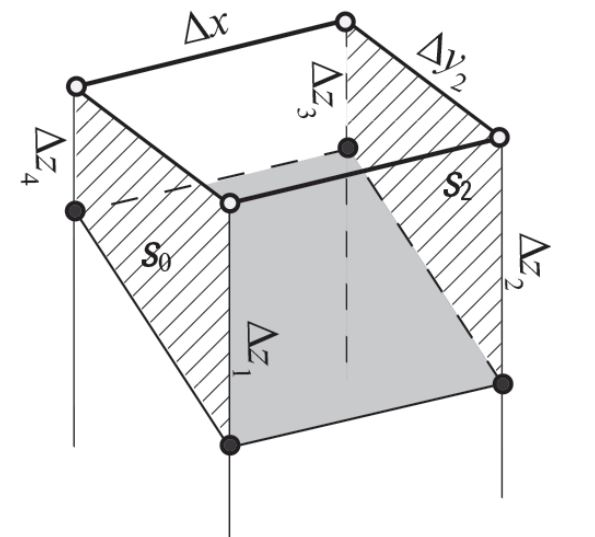
\includegraphics[width=0.5\textwidth]{complete_column.JPG}
\caption{Representaci\'on gr\'afica de una columna completamente contenida dentro de una esfera de evaluaci\'on. Fuente: Manual de usuario de Scoops3D.}
\label{fig:Interfaz de usuario}
\end{figure}

Dado que scoops3D tiene en cuenta todas aquellas columnas que contengan 2 vertices al interior de la esfera de busqueda, es posible que solo una parte de la columna este contenida dentro de dicha esfera, caso en el cual el volumen de dicha parte incluida debe ser calculado.
En este caso y partiendo de la figura 3.2, se toma un plano intermedio $ S_{1} $ entre los planos $ S_{0} $ y $ S_{2} $

En los casos en los que una columna es contenida es su totalidad, es decir, que sus planos  paralelos $S_{0}$ y $S_{2}$ tienen igual area. el volumen (\textit{V}) estara dado por 

$$\textit{V}= (1/6)\vartriangle \textit{x}(S_{0} + 4S_{1} + S_{2})$$

donde el area del plano $\textit{S}_{0}$ estara dada por
$$ \textit{S}_{0} = (1/2)(\vartriangle z_{1} +\vartriangle z_{1})+\vartriangle \textit{y}_{1}  $$

y el area del plano paralelo $\textit{S}_{0}$
$$ \textit{S}_{2} = (1/2)(\vartriangle z_{2} +\vartriangle z_{3})+\vartriangle \textit{y}_{2}  $$

Finalmente, el peso $W$ de la columna estara representado por

$$\textit{W} = \int \textit{V} \gamma (\textit{z}) \textit{dz} $$

Donde $ \gamma$ es el peso unitario del suelo, el cual puede variar con la profundidad $\textit{z}$

En general, los m\'etodos de equilibrio l\'imite definen el Factor de seguridad (F) como la relaci\'on entre las fuerzas resistentes  \textit{s} y las fuerzas actuantes $\tau$

$$F =\frac{\textit{s}}{\tau}$$

Donde F inferior a uno (1) indica inestabilidad. Para \'areas definidas, como el \'area en la base de cada columna (\textit{A})

La fuerza actuante (\textit{T}) sobre \textit{A} estar\'a dada por

$$\textit{T}=\left(\frac{1}{\textit{A}}\right)\int_{\textit{A}}^{} \frac{\textit{s}\textit{A}}{\textit{F}} \textit{dA}$$

Discretizando las componentes\textit{i} y \textit{j} correspondientes a las fuerzas resistentes \textit{x} y \textit{y} respectivamente, se tiene.

$$\textit{T} = \frac{1}{\textit{F}} \Sigma\textit{s}_{\textit{i,j}} \textit{A}_{\textit{i,j}}$$

\begin{center}


\begin{tabular}{|c|c|c|c|c|c|c|c|c|c|}
\hline 
\textit{i,j} & \textit{i,j} & \textit{i,j} & \textit{i,j} & \textit{i,j} & \textit{i,j} & \textit{i,j} & \textit{i,j} & \textit{i,j} & \textit{i,j} \\ 
\hline 
\textit{i,j}& \textit{i,j}& \textit{i,j} & \textit{i,j} &\textit{i,j} & \textit{i,j} & \textit{i,j} & \textit{i,j} & \textit{i,j} & \textit{i,j} \\ 
\hline 
\textit{i,j} & \textit{i,j} & \textit{i,j} & \textit{i,j} & \textit{i,j} & \textit{i,j} & \textit{i,j} & \textit{i,j} & \textit{i,j} & \textit{i,j} \\ 
\hline 
\textit{i,j} & \textit{i,j} & \textit{i,j} & \textit{i,j} & \textit{i,j} & \textit{i,j} & \textit{i,j} & \textit{i,j} & \textit{i,j} & \textit{i,j} \\ 
\hline 
\textit{i,j} & \textit{i,j} & \textit{i,j} & \textit{i,j} & \textit{i,j} & \textit{i,j} & \textit{i,j} & \textit{i,j} & \textit{i,j} & \textit{i,j} \\ 
\hline 
\textit{i,j}& \textit{i,j}& \textit{i,j}& \textit{i,j} & \textit{i,j}& \textit{i,j}& \textit{i,j} & \textit{i,j} &\textit{i,j} & \textit{i,j} \\ 
\hline 
\textit{i,j} &\textit{i,j} & \textit{i,j} & \textit{i,j} & \textit{i,j} & \textit{i,j}& \textit{i,j}& \textit{i,j} & \textit{i,j}& \textit{i,j} \\ 
\hline 
\textit{i,j} & \textit{i,j}& \textit{i,j}& \textit{i,j} & \textit{i,j} & \textit{i,j} & \textit{i,j} & \textit{i,j}& \textit{i,j} & \textit{i,j}\\ 
\hline 
1,2 & 2,2 & \textit{i,j} & \textit{i,j} & \textit{i,j} & \textit{i,j}& \textit{i,j} & \textit{i,j} & \textit{i,j}& \textit{i,j}\\ 
\hline 
1,1 & 2,1 & \textit{i,j}& \textit{i,j} & \textit{i,j} & \textit{i,j} & \textit{i,j} & \textit{i,j}& \textit{i,j} & \textit{i,j}\\ 
\hline 
\end{tabular} 
\end{center}
La columna $\textit{i}=1$ y $\textit{j}=1$ ser\'a aquella ubicada en la posici\'on del p\'ixel en la esquina inferior izquierda del DEM.

El equilibrio de momentos se calcula a lo largo de un eje rotacional basado en el centro de la esfera de falla, dicho eje es horizontal y normal a la direcci\'on potencial de falla.
El momento actuante est\'a direccionado principalmente por la fuerza de la gravedad (\textit{W})
$$a_{i,j}=R_{i,j}\sin \alpha_{i,j}$$ 

Donde $\textit{R}_{i,j}$ es la distancia desde el centro de la esfera hasta el centro del \'area $\textit{A}$ en la base de la columna, $\alpha_{i,j}$ es el buzamiento aparente del plano de \'area (\textit{A}) visto desde la posici\'on del centro de la esfera. En $\textit{R}_{i,j}$ se puede apreciar una de las principales diferencias entre el an\'alisis de equilibrio limite en 2D y 3D, ya que en 3D dicha distancia siempre es variable, por lo cual el momento actuante ($\textit{M}_{act}$) de cada columna debe calcularse independientemente, para lo cual se usa la expresi\'on:

$$\textit{M}_{act}=\Sigma \textit{R}_{i,j}\textit{W}_{i,j}\sin\alpha_{i,j}  $$

El momento resistente($\textit{M}_{r}$)  est\'a representado por la sumatoria de los productos de esfuerzos cortantes en la parte inferior de cada columna.

$$\textit{M}_{Total}= \Sigma \textit{R}_{i,j}\frac{\textit{s}_{i,j}\textit{A}_{i,j}}{\textit{F}}  $$
por lo que al reemplazar $\textit{s}_{i,j}$ 

$$ {M}_{Total} = \Sigma \textit{R}_{i,j} \frac{\textit{C}_{i,j}\textit{A}_{i,j}+(\textit{N}_{i,j}-\textit{U}_{i,j}\textit{A}_{i,j})\tan\phi_{i,j}}{\textit{F}} $$

Donde $\textit{N}_{i,j}$ es la fuerza normal correspondiente a cada columna.\\

El momento de equilibrio para una columna individual estar? dada entonces por la expresion.
$$ \Sigma \textit{M}= \Sigma \textit{R}_{i,j} \frac{\textit{c}_{i,j}\textit{A}_{i,j}+(\textit{N}_{i,j}-\textit{u}_{i,j}\textit{A}_{i,j})\tan\phi _{i,j}}{F}-\Sigma \textit{W}_{i,j}\textit{R}_{i,j}\sin \alpha _{i,j} $$

Por lo que el factor de seguridad \textit{F} Est\'a dado por:

$$\textit{F}_{i,j}=  \frac{\Sigma \textit{R}_{i,j}(\textit{c}_{i,j}\textit{A}_{i,j}+(\textit{N}_{i,j}-\textit{u}_{i,j}\textit{A}_{i,j})\tan \phi _{i,j}}{\Sigma \textit{W} _{i,j}(\textit{R} _{i,j}\sin\alpha _{i,j})}  $$

